\chapter{Experiments}

All the experiments have been executed on the Devbox cluster provided by TIB and on a single Nvidia RTX-3090 GPU with 24 GB vRAM, 32 virtual CPUs, and 500GB main memory. 

\section{Subsampling and distinct frame detection}

As there were no datasets to test the distinct frame detection, 6 video samples of four three types were randomly sampled from the TIB AV-Portal \cite{noauthor_tib_nodate} and Youtube. The videos are typical live lecture recordings with a professor writing on the screen, digital presentations with slides, and videos of lectures handwritten on paper. The videos have different lengths, framerates, resolutions, and lighting conditions. The results of the experiments are shown in table \ref{tab:uniqueframedetresults}.

\begin{table}[!ht]
    \centering
    \caption{Results of running the distinct frame detection algorithm on six videos of different types, total frames is the number of frames in the video before subsampling, skip frames is the number of frames processed by the distinct frame detection algorithm, unique frames is the number of frames chosen by the algorithm}
    \begin{tabular}{|c|c|c|c|c|}
    \hline
        \textbf{type} & \textbf{total frames} & \textbf{skip frames} & \textbf{unique frames} & \textbf{reduction} \\ \hline
        writing on paper & 4604 & 192 & 10 & \textbf{0.95} \\ \hline
        writing on paper & 11363 & 455 & 287 & 0.37 \\ \hline
        writing on board board & 40859 & 1635 & 980 & 0.40 \\ \hline
        writing on board & 26052 & 1043 & 1016 & \textbf{0.03} \\ \hline
        presentation & 5807 & 233 & 11 & \textbf{0.95} \\ \hline
        presentation & 19156 & 767 & 61 & 0.92 \\ \hline
    \end{tabular}
    \label{tab:uniqueframedetresults}
\end{table}

As evident from the results, subsampling drastically reduces the number of frames that must be processed in the first stage of filtering. The frames chosen by the subsampling are then passed to the distinct frame detection algorithm. The reduction in the number of frames that must be processed by later stages of the pipeline thanks to the distinct frame detection ranges from $3\%$ to $95\%$. The best reduction of $95\%$ is obtained when applied to presentation recordings; this is because the algorithm measures pixel-wise differences between consecutive frames, and recordings of presentations usually have all text already written and have clear transitions between successive slides. On the other hand, if the text is being actively written with the writer's hand covering parts of the image and coming in and out of the picture, leading to big differences between the images as is the case with videos of writing on paper, then the performance of the algorithm will drop to $37\%$. This is emphasized in recordings of lectures where the camera might follow the teacher and zoom in and out on a specific region of the board, leading to even bigger differences between frames.

The algorithm processes frames with $1024\times576$ pixel resolution at a speed of 26 FPS, meaning that it takes one minute on average to process 26 minutes of video (after subsampling). This is fast enough to be executed as a pre-stage to the main text localization stage, which, depending on the selected method, might be pretty slow, as we'll see in the next section.

\section{Text localization methods}

At this stage, the performance of the different text detection methods was tested.

\begin{table}[!ht]
    \centering
    \caption{Performance of different text localization methods tested on LVDB test set. ResNet 18 and 50 means that the model's backbone is a ResNet 18 or 50 CNN. The rows are sorted based on the F1@.5 score.}
    \begin{tabular}{|l|l|l|l|l|}
    \hline
        Model name & Precision@.5 & Recall@.5 & F1@.5 (H-mean) & FPS \\ \hline
        PSENet & 0.8107 & 0.5637 & 0.665 & 3 \\ \hline
        FCENet & 0.8115 & 0.7116 & 0.7583 & 1 \\ \hline
        Mask R-CNN & 0.7902 & 0.7893 & 0.7898 & 5 \\ \hline
        PANet & 0.869 & 0.7638 & 0.813 & 12 \\ \hline
        DBNet (ResNet 18) & 0.8611 & 0.7957 & 0.8271 & 11 \\ \hline
        DBNet (ResNet 50) & 0.8334 & 0.8225 & 0.8279 & 9 \\ \hline
        DBNet++ (ResNet 50) & 0.887 & 0.8109 & 0.8473 & 9 \\ \hline
        YOLOv7 & \textbf{0.887} & \textbf{0.841} & \textbf{0.864} & \textbf{277} \\ \hline
    \end{tabular}
    \label{tab:text_loc_results}
\end{table}

The results are a bit surprising as the best model YOLOv7 was not designed specifically to be a text detection model like the others. On the LVDB test set, YOLOv7 reaches an F1@.5 score of $86.4\%$, $1.67$ percentage points better than the runner-up DBNet++. YOLOv7 is a state-of-the-art object detection method built to locate objects in complex scenes, so detecting a single object class (text) in somewhat similar scenes is not that big of a challenge. On the other hand, DBNet++ was also released in 2022 but focused on detecting text of different shapes and forms rather than regular text but in the case of lecture videos, most of the text is horizontal and has no weird shapes like in logos. Though they both have similar Precision of $88.7\%$ at $50\%$ IOU threshold, YOLOv7 has higher Recall which means it can find more of the text in the image. Added to that, YOLO has been designed from the ground up to run in real-time and as fast as possible allowing it to achieve $23$ times higher FPS than the best model PANet with 277 FPS. That high speed is exceptionally important for processing the hundreds or thousands of images selected by the unique frame detection algorithm.
A sample of predicted bounding boxes by YOLOv7 is shown in \hyperref[exp:yolo_pred]{this figure}.

\begin{figure}[H]
        \centering
        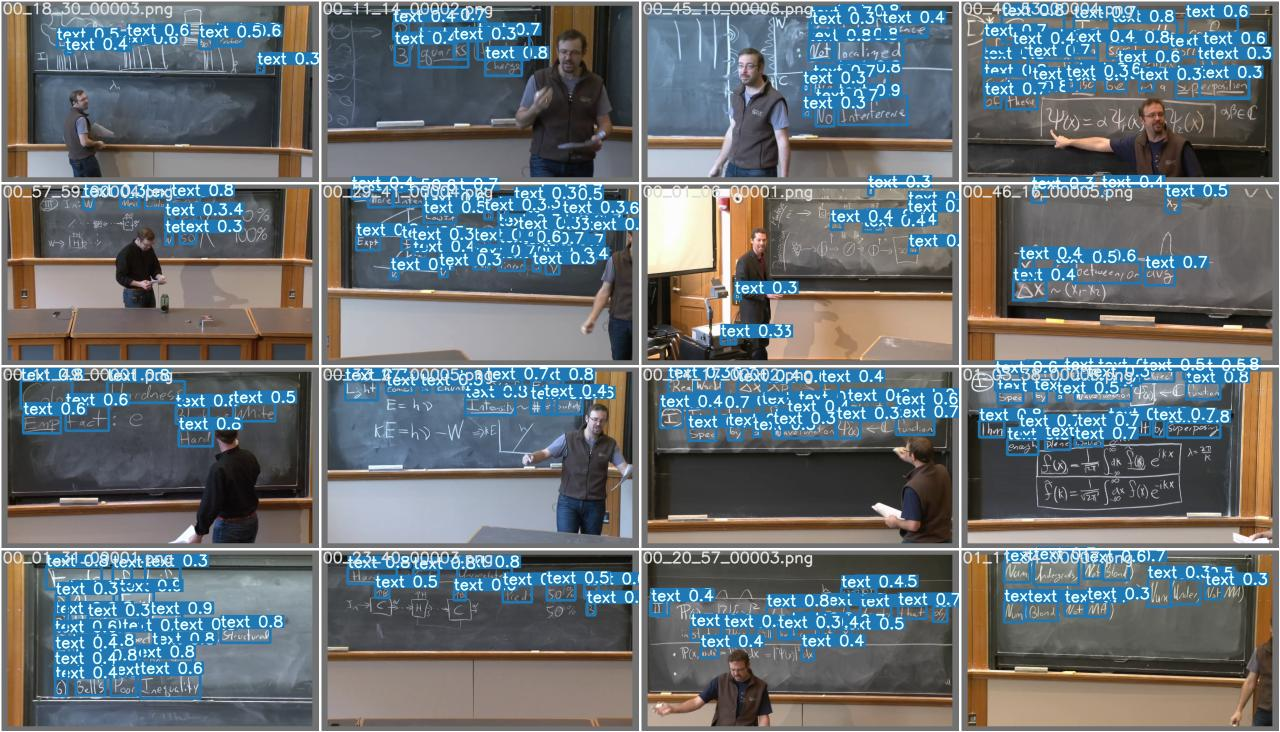
\includegraphics[width=140mm]{figures/test_batch0_pred.jpg}
        \caption{YOLOv7 predictions on LVDB test set}
        \label{exp:yolo_pred}
\end{figure}

\section{Text recognition methods}

\begin{table}[!ht]
    \centering
    \caption{Performance of different text recognition methods tested on LVDB test set sorted based on 1-N.E.D then word accuracy then FPS}
    \begin{tabular}{|l|l|l|l|l|l|}
    \hline
        Model name & 1-N.E.D & Word accuracy & Char recall & Char precision & FPS \\ \hline
        tesseract oem 0 & 0.4139 & 0.2333 & 0.5561 & 0.7 & 25 \\ \hline
        tesseract oem 2 & 0.5084 & 0.2747 & 0.6714 & 0.7814 & 26 \\ \hline
        tesseract oem 1 & 0.5379 & 0.2942 & 0.7028 & 0.7899 & 35 \\ \hline
        SAR & 0.8319 & 0.6896 & 0.8738 & 0.894 & 116 \\ \hline
        NRTR\_1/16-1/8 & 0.8765 & 0.7764 & 0.9283 & 0.932 & 276 \\ \hline
        ABINet & 0.8774 & 0.7574 & 0.9178 & 0.9033 & 310 \\ \hline
        NRTR\_1/8-1/4 & 0.8791 & 0.7816 & 0.9303 & 0.9315 & 197 \\ \hline
        SATRN (small) & 0.8807 & 0.7761 & 0.9261 & 0.9276 & 300 \\ \hline
        MASTER & 0.8811 & 0.777 & 0.9237 & 0.9305 & 156 \\ \hline
        SATRN & 0.8891 & 0.7914 & 0.9311 & 0.935 & 166 \\ \hline
        PARSeq & \textbf{0.8929} & \textbf{0.7955} & \textbf{0.9364} & \textbf{0.9388} & \textbf{770} \\ \hline
    \end{tabular}
    \label{tab:text_rec_results}
\end{table}

In the case of text recognition methods, the performance of all the models except for tesseract is pretty high with most of the models having 1-N.E.D higher than $83\%$, word accuracy higher than $77\%$, and character recall and precision higher than $87\%$.

The real difference between these models shows up in their inference speed. FPS in these tests corresponds to the number of words per second the model was able to process given that they were all tested on the same hardware and with the maximal batch size that can fit into GPU memory. Two models shine when it comes to speed: ABINet and PARSeq. 

What the ABINet model lacks in accuracy and recall it makes up for it in speed by processing $310$ words from the test set per second on average. But because it requires an external language model that has to be set up and trained separately from the rest of the model using ABINet in a production environment is a hustle and doesn't provide an easy way of continuously training the model as new data comes in.

The \hyperref[parseq]{PARSeq} model released in September 2022, achieves SOTA performance on known datasets like ICDAR-2013, ICDAR-2015, CUTE80, SVT, SVTP, and IIIT5K \cite{bautista_scene_2022}. It also has the best 1-N.E.D with $89.29\%$ and the best word accuracy of $79.55\%$.
The test samples for which PARSeq incorrectly transcribes had either an incorrect ground-truth label or they were hard to read even by the average human reader; figure \ref{exp:parseq_wrong_recog} shows examples of misspelled words.
It also reaches an inference speed of $770$ words per second; double the inference speed of the runner-up ABINet. This high performance is thanks to its simple design with no convolutional layers (ViT encoder) and the integration of the language model in the multi-modal decoder. Allowing it to use a batch size of up to 2000 images (cropped-out words) on a 24GB RTX-3090.

Independent of which model was tested, the results have shown that the recognition accuracy also depends on whether the character's case and punctuation are considered when calculating the metrics. All of the models had an increase in their 1-N.E.D metric when uppercase characters and symbols were ignored as shown in table \ref{tab:text_rec_results_ignore}. A close examination of the SynthText, MJSynth, and LVDB datasets reveals the cause of this disparity in performance between the performance with and without punctuation. First, the models fail to recognize different symbols because of the lack of punctuation in the two synthetic datasets SynthText and MJSynth on which they were pre-trained. Second, taking a sample from the test set of LVDB with punctuation, it becomes obvious that some ground-truth labels are wrong and don't include punctuation as shown in figure \ref{exp:parseq_wrong_recog}.

\begin{table}[!ht]
    \centering
    \caption{Performance of text recognition methods when ignoring case and punctuation}
    \begin{tabular}{|l|l|l|l|}
    \hline
        Model name & 1-N.E.D & 1-N.E.D ignore case & 1-N.E.D ignore case and punctuation \\ \hline
        tesseract oem 0 & 0.4139 & 0.5066 & 0.5235 \\ \hline
        tesseract oem 2 & 0.5084 & 0.613 & 0.6264 \\ \hline
        tesseract oem 1 & 0.5379 & 0.6428 & 0.6536 \\ \hline
        SAR & 0.8319 & 0.8478 & 0.8521 \\ \hline
        NRTR\_1/16-1/8 & 0.8765 & 0.9004 & 0.9058 \\ \hline
        ABINet & 0.8774 & 0.8782 & 0.8813 \\ \hline
        NRTR\_1/8-1/4 & 0.8791 & 0.9024 & 0.9082 \\ \hline
        SATRN\_sm & 0.8807 & 0.8982 & 0.9033 \\ \hline
        MASTER & 0.8811 & 0.8974 & 0.902 \\ \hline
        SATRN & 0.8891 & 0.905 & 0.9097 \\ \hline
        PARSeq & 0.8929 & 0.9123 & 0.9173 \\ \hline
    \end{tabular}
    \label{tab:text_rec_results_ignore}
\end{table}

\begin{figure}[H]
        \centering
        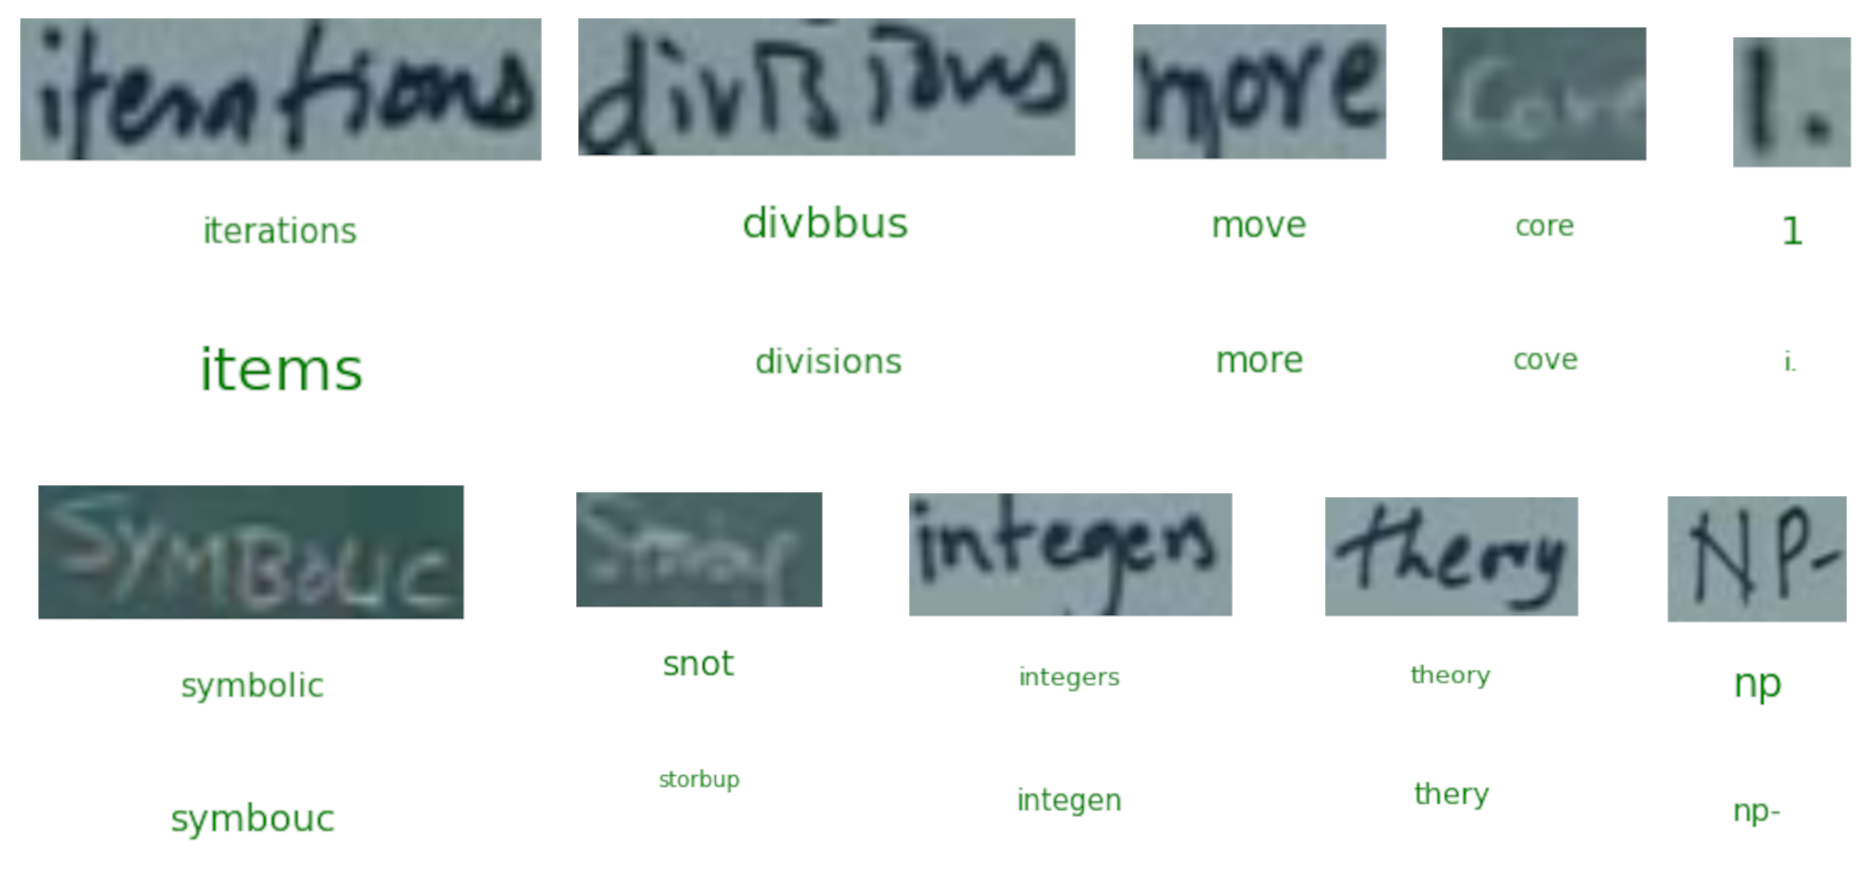
\includegraphics[width=140mm]{figures/parseq_wrong_recog.png}
        \caption{Examples of incorrectly transcribed words by PARSeq. The ground-Truth label is on top and prediction is on the button.}
        \label{exp:parseq_wrong_recog}
\end{figure}

\section{Context-free error correction}

The dictionary-based error correction using the SymSpell algorithm was tested using the PARSeq model and has proven to have little to no effect on the recognition accuracy. On the LVDB test set PARSeq's word accuracy increased slightly from $79.55\%$ to $79.84\%$. The reason why there is a minimal improvement in performance in contrast to what one might expect becomes clear when the number of predictions to which the correction algorithm is applied is more closely investigated. The correction algorithm is only triggered when the predicted word is not found in the dictionary; for PARSeq during testing, those came out to be $9979$ out of $41248$ total test samples. Also, the correction was only triggered on words longer than 3 characters; this minimum word length has been chosen because I found out during testing that the model's performance got worse when also considering short words. This is caused by the SymSpell algorithm changing valid words like "b" to "a" because the letter "a" was more frequent in the English language than the letter "b". So out of the $9979$ words, there are only $2968$ words that are longer than three characters long. And out of those only $1903$ were corrected by the SymSpell algorithm. The rest $1065$ predictions were not corrected because an equivalent word with an edit distance of less than two was not found in the dictionary. A sample of the OOV words reveals that not all of them are necessarily wrong, but most are scientific terms or entity names that weren't listed in the dictionary. For example "backoff" (in the context of algorithms), "IETF" (Internet Engineering Task Force), "sizeof" (in programming languages), "1990s", and "6x10" are all correct words but are classified as OOV words and count towards that total of $1065$ not corrected words.